\documentclass[conf]{../paper/new-aiaa}
%\documentclass[journal]{new-aiaa} for journal papers
\usepackage[utf8]{inputenc}

\usepackage{graphicx}
\usepackage{amsmath}
\usepackage[version=4]{mhchem}
\usepackage{siunitx}
\usepackage{longtable,tabularx}
\usepackage{footnote}
\usepackage{mhchem}
\usepackage{physics}
\usepackage{array,makecell,booktabs}
\newcolumntype{M}[1]{>{\centering\arraybackslash}m{#1}}
\newcommand{\head}[2]{\multicolumn{1}{>{\centering\arraybackslash}p{#1}}{#2}}
\usepackage[super]{nth}
\usepackage{multirow}
\makesavenoteenv{tabular}
\setlength\LTleft{0pt} 
\DeclareMathOperator*{\mean}{mean}

\graphicspath{{figures/}}

\title{Strategies for Re-Use of Launch Vehicle First Stages: Uncertainty Quantification}

\author{Matthew T. Vernacchia \footnote{Research Assistant, Department of Aeronautics and Astronautics, 77 Massachusetts Avenue, AIAA Student Member.}
and Kelly J. Mathesius  \footnote{Research Assistant, Department of Aeronautics and Astronautics, 77 Massachusetts Avenue, AIAA Student Member.}}
\affil{Massachusetts Institute of Technology, Cambridge, MA, 02139}


\begin{document}

\maketitle

\section{Performance-Related Uncertainties}

\subsection{Technology Uncertainties}
Uncertainties on the performance factors which we choose to group as the "technology choice": i.e. the specific impulse and inert mass fractions of each stage $c_1, c_2, E_1, E_2$.

Note this is not uncertainty about what the technology choice is - we assume that is given. Rather, given a technology choice (e.g. kerosene fuel, gas generator engine cycle, and aluminum alloy tanks), what is the remaining uncertainty in Isp and inert mass fraction?

\subsubsection{Specific Impulse}
The specific impulse is largely determined by the choice of propellant and engine cycle. However, there are still variations in nominal specific impulse between different engines using the same propellant and cycle and variations away from the nominal specific impulse in the operation of a given engine. These variations contribute to uncertainty in the performance of a new launch vehicle design.

We divide the sources of variation in specific impulse into two categories:
\begin{itemize}
    \item \emph{variation in nominal $I_{sp}$} -  This captures variations in nominal specific impulse between different engines using the same propellant and cycle. Contributing factors (which may be uncertain at the outset of an engine development project) include chamber pressure, mixture ratio, expansion ratio, and injector $c^*$ efficiency.
    \item \emph{variation in operation} -  This captures variations away from the nominal specific impulse in the operation of a given engine. Contributing factors which may vary between missions include throttling, mixture ratio control, and ambient pressure on different possible trajectories.
\end{itemize}

Uncertainty in nominal $I_{sp}$ only exists if a new engine will be developed for the launch vehicle, or if the engine selection is yet to be made. For a particular launch vehicle, the nominal specific impulse is known once an engine is selected or developed. However, we wish our performance predictions to be representative of the population of engines using a particular technology, and thus include the variation in nominal specific impulse as an uncertainty in the model. TODO.

We model the variation in nominal $I_{sp}$ by examining a sample of existing and historical launch vehicle engines (see Table \ref{tab:engine_historical_trends}; we believe that this is a comprehensive sample of all hydrogen and kerosene engines used for space launch). First, we must determine whether there are historical trends in the performance data. If there were a strong historical trend towards improving performance, then a sample of historical engines would not be representative of the performance in modern and near-future engines. However, liquid propulsion has been a mature field for some time \cite{hist_lpre}, and Figure \ref{fig:engine_historical_trends} shows no clear correlation between performance and year of first flight after 1975. Thus these engines are likely representative of the performance of contemporary and near-future engines.


\begin{figure}[hbt!]
    \centering
    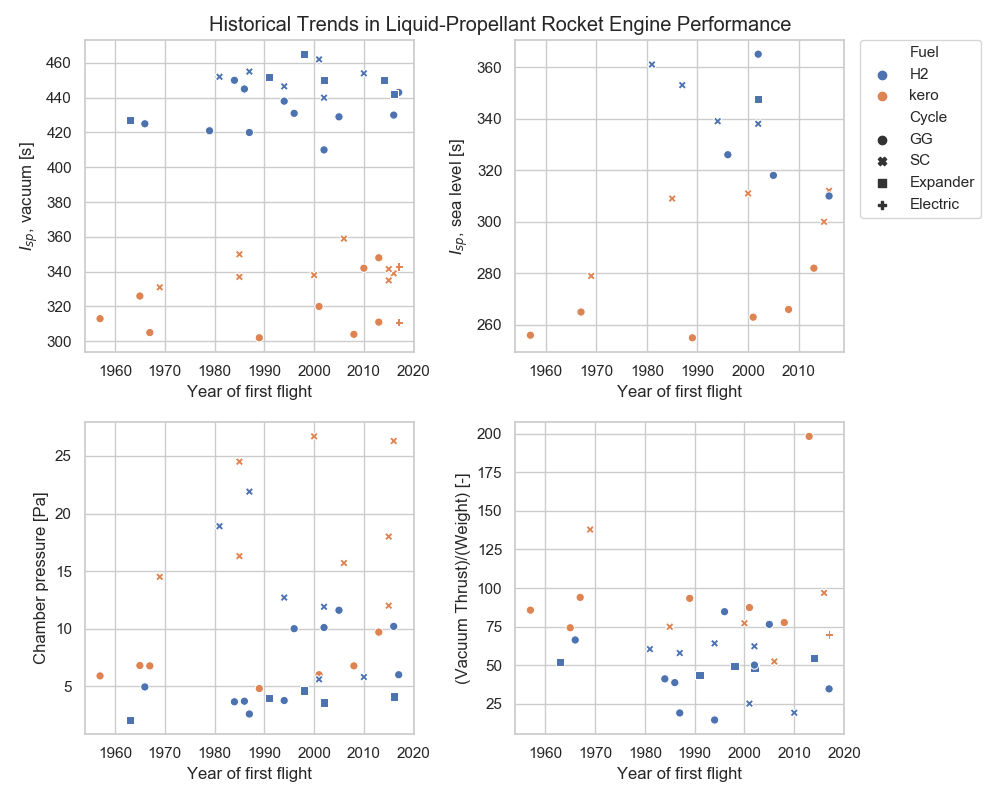
\includegraphics[width=1\textwidth]{engine_trends/engine_historical_trends}
    \caption{\label{fig:engine_historical_trends} Historical trends in engine performance. After 1975, there is no clear correlation of performance with time, thus these engines are likely representative of the performance of contemporary and near-future engines.}
\end{figure}

\begin{figure}[hbt!]
    \centering
    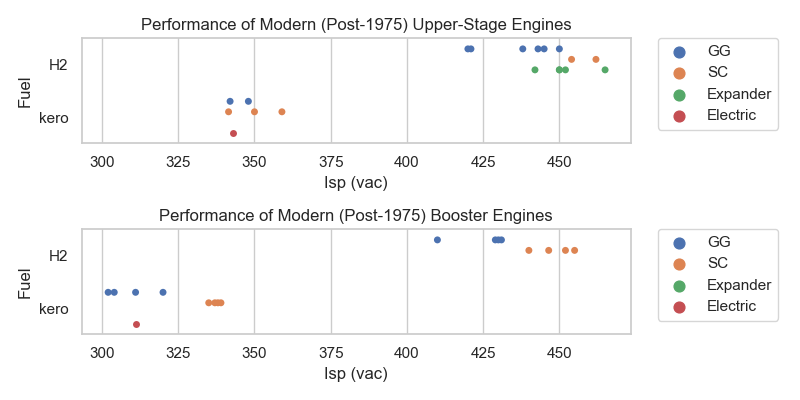
\includegraphics[width=1\textwidth]{engine_trends/engine_isp_dist}
    \caption{\label{fig:engine_isp_dist} Distribution of vacuum specific impulse of modern liquid propellant rocket engines, categorized by fuel and engine cycle. Unsurprisingly, hydrogen fuel and closed cycle (staged combustion or expander) engines have higher $I_{sp}$. The $I_{sp}$ spread within each category is \SIrange{6}{30}{\second}}
\end{figure}

\begin{table}
    \caption{\label{tab:engine_historical_trends} Examples of liquid propellant rocket engines used for space launch.}
    \centering
    \small
    \begin{tabular}{llllrrrrr}
\toprule
{} &      Use &  Fuel &     Cycle & \head{1.5cm}{$I_{sp}$, vacuum [s]} & \head{1.5cm}{$I_{sp}$, sea level [s]} & \head{1.5cm}{Chamber pressure [MPa]} & \head{1.5cm}{Thrust \slash Weight [-]} & \head{1.5cm}{Year of first flight} \\
Engine            &          &       &           &           &          &                  &                     &                      \\
\midrule
CE-20             &    Upper &    H2 &        GG &       443 &      - &              6.0 &                  35 &                 2017 \\
CE-7.5            &    Upper &    H2 &        SC &       454 &      - &              5.8 &                  19 &                 2010 \\
F-1               &  Booster &  kero &        GG &       305 &      265 &              6.8 &                  94 &                 1967 \\
HM7A              &    Upper &    H2 &        GG &       421 &      - &              - &                 - &                 1979 \\
HM7B              &    Upper &    H2 &        GG &       445 &      - &              3.7 &                  39 &                 1986 \\
J-2               &    Upper &    H2 &        GG &       425 &      - &              4.9 &                  66 &                 1966 \\
LE-5              &    Upper &    H2 &        GG &       450 &      - &              3.6 &                  41 &                 1984 \\
LE-5A             &    Upper &    H2 &  Expander &       452 &      - &              4.0 &                  44 &                 1991 \\
LE-5B             &    Upper &    H2 &  Expander &       450 &      348 &              3.6 &                  48 &                 2002 \\
LE-7              &  Booster &    H2 &        SC &       446 &      339 &             12.7 &                  64 &                 1994 \\
LE-7A             &  Booster &    H2 &        SC &       440 &      338 &             11.9 &                  62 &                 2002 \\
Merlin 1C         &  Booster &  kero &        GG &       304 &      266 &              6.8 &                  78 &                 2008 \\
Merlin 1C Vacuum  &    Upper &  kero &        GG &       342 &      - &              - &                 - &                 2010 \\
Merlin 1D         &  Booster &  kero &        GG &       311 &      282 &              9.7 &                 198 &                 2013 \\
Merlin 1D Vacuum  &    Upper &  kero &        GG &       348 &      - &              - &                 - &                 2013 \\
NK-33             &  Booster &  kero &        SC &       331 &      279 &             14.5 &                 138 &                 1969 \\
RD-0110           &    Upper &  kero &        GG &       326 &      - &              6.8 &                  74 &                 1965 \\
RD-0120           &  Booster &    H2 &        SC &       455 &      353 &             21.9 &                  58 &                 1987 \\
RD-0124           &    Upper &  kero &        SC &       359 &      - &             15.7 &                  52 &                 2006 \\
RD-107            &  Booster &  kero &        GG &       313 &      256 &              5.9 &                  86 &                 1957 \\
RD-107A           &  Booster &  kero &        GG &       320 &      263 &              6.0 &                  87 &                 2001 \\
RD-120            &    Upper &  kero &        SC &       350 &      - &             16.3 &                  75 &                 1985 \\
RD-170, RD-171    &  Booster &  kero &        SC &       337 &      309 &             24.5 &                  75 &                 1985 \\
RD-180            &  Booster &  kero &        SC &       338 &      311 &             26.7 &                  77 &                 2000 \\
RD-181            &  Booster &  kero &        SC &       339 &      312 &             26.3 &                  97 &                 2016 \\
RD-56 (KDV-1)     &    Upper &    H2 &        SC &       462 &      - &              5.6 &                  25 &                 2001 \\
RL10A-3           &    Upper &    H2 &  Expander &       427 &      - &              2.1 &                  52 &                 1963 \\
RL10B-2           &    Upper &    H2 &  Expander &       465 &      - &              4.6 &                  49 &                 1998 \\
RL10C-1           &    Upper &    H2 &  Expander &       450 &      - &              - &                  55 &                 2014 \\
RS-25 (SSME)      &  Booster &    H2 &        SC &       452 &      361 &             18.9 &                  60 &                 1981 \\
RS-27A            &  Booster &  kero &        GG &       302 &      255 &              4.8 &                  93 &                 1989 \\
RS-68             &  Booster &    H2 &        GG &       410 &      365 &             10.1 &                  50 &                 2002 \\
Rutherford        &  Booster &  kero &  Electric &       311 &      - &              - &                  70 &                 2017 \\
Rutherford Vacuum &    Upper &  kero &  Electric &       343 &      - &              - &                 - &                 2017 \\
Vulcain 1         &  Booster &    H2 &        GG &       431 &      326 &             10.0 &                  85 &                 1996 \\
Vulcain 2         &  Booster &    H2 &        GG &       429 &      318 &             11.6 &                  76 &                 2005 \\
YF-100            &  Booster &  kero &        SC &       335 &      300 &             18.0 &                 - &                 2015 \\
YF-115            &    Upper &  kero &        SC &       342 &      - &             12.0 &                 - &                 2015 \\
YF-73             &    Upper &    H2 &        GG &       420 &      - &              2.6 &                  19 &                 1987 \\
YF-75             &    Upper &    H2 &        GG &       438 &      - &              3.8 &                  15 &                 1994 \\
YF-75D            &    Upper &    H2 &  Expander &       442 &      - &              4.1 &                 - &                 2016 \\
YF-77             &  Booster &    H2 &        GG &       430 &      310 &             10.2 &                 - &                 2016 \\
\bottomrule
\end{tabular}

    \\
    All listed engines use liquid \ce{O2} oxidizer. GG = gas generator, SC = staged combustion. Data from \cite{hist_lpre,wiki:OrbitalEngines, Falcon9}.
\end{table}

Next, we need to quantify the uncertainty due to variation in operation. The listed specific impulse values are typically measured at design conditions; we expect that off-design operation could lower these values by 2\%. For \nth{2} (upper) stage engines, which operate in near vacuum, this is the end of the story. For booster engines, there is also a large variation in specific impulse due the effects of altitude. Our performance model requires $c_1$ to be the \emph{effective} \nth{1} stage specific impulse, averaged over the altitudes at which an engine operates. As a crude estimate, we will assume that the effective specific impulse is the mean of the sea level and vacuum values:

\[
    c_1 \approx g_0 \left( \frac{I_{sp, vac} + I_{sp, SL}}{2} \right)
\]

This crude estimate results in surprisingly descent performance predictions \cite{Alber2012}. 

Our performance model needs distributions on $c_1$ and $c_2$, which represent the possible variation in those parameters for a given technology choice. We arbitrarily choose to use triangular distributions, which are commonly used as a rough guess description when limited sample data is available. We will choose the parameters of the distributions based on the historical engine data. We fit a different distribution for each choice of propellant and engine cycle.

For upper stage engines, the distribution parameters are:
\[
 min = 0.98 g_0 \min_{e \in S}(I_{sp, vac}^{e})
\]
\[
 max = g_0 \max_{e \in S}(I_{sp, vac}^{e})
\]
\[
 mode = g_0 \mean_{e \in S}(I_{sp, vac}^{e})
\]

where $S$ is the set of historical engines matching the given propellant and cycle, and $e$ is an engine from that set.

For booster engines, the mean of the vacuum and sea level $I_{sp}$ is used, and the bounds of the distribution are spread by an additional 3\% to account for the crudity of this estimate:
\[
 min = 0.95 g_0 \min_{e \in S}\left( \frac{I_{sp, vac}^e + I_{sp, SL}^e}{2} \right)
\]
\[
 max = 1.03 g_0 \max_{e \in S}\left( \frac{I_{sp, vac}^e + I_{sp, SL}^e}{2} \right)
\]
\[
 mode = g_0 \mean_{e \in S}\left( \frac{I_{sp, vac}^e + I_{sp, SL}^e}{2} \right)
\]

\subsubsection{Inert mass fraction - expendable baseline}
The inert mass fraction expendable baselines, $E_1, E_2$, represent the lower limit of achievable inert mass fraction for a particular technology choice.
The values of $E_1, E_2$ are uncertain and hard to predict from first principles, as they result from a complicated engineering process. However, we can make an informed guess as to what is possible by examining historical trends in launch vehicle stages.

We compiled a sample of historical and active stages which have been sucessfully used in space launch vehicles; the data is drawn mainly from \cite{Isakowitz2004}. We segregate the data into boosters (first stages) and upper stages, as these have different structural design requirements. The present analysis only considers sequentially-staged launch vehciles, so we exclude boosters which cannot lift off under their own thrust.

 First, we must determine whether there are historical trends in the inert mass fraction data. If there were a strong historical trend towards improving inert mass fraction, then a sample of historical stages would not be representative of the performance in modern and near-future stages. Examining Figure \ref{fig:stage_historical_trends}:
 \begin{itemize}
    \item For hydrogen upper stages there is no clear historical trend.
    \item For kerosene upper stages inert mass fraction has declined with time.
    \item For hygrogen boosters, there is only one example capable of liftoff under its own thrust (Delta IV Common Booster Core), so no historical trends can be observed.
    \item For kerosene boosters, there is no clear historical trend.
\end{itemize}

% TODO include table

\begin{figure}[hbt!]
    \centering
    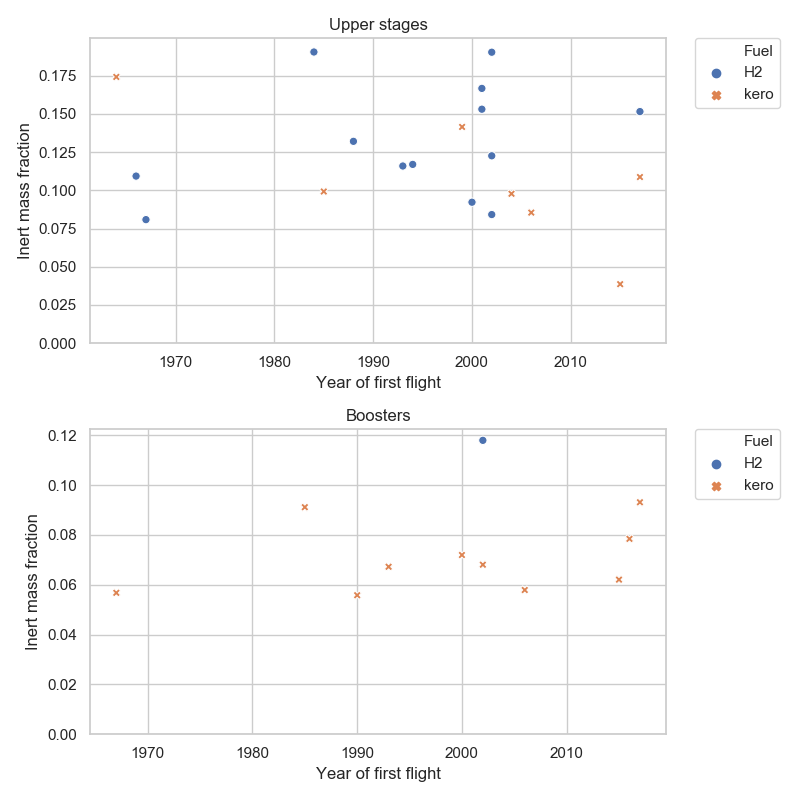
\includegraphics[width=1\textwidth]{stage_trends/stage_historical_trends}
    \caption{\label{fig:stage_historical_trends} Historical trends in stage inert mass. There are no clear trends with time, excepting the declining inert mass fraction of kerosene/\ce{O2} upper stages.}
\end{figure}

Next, we consider the relation between stage inert mass fraction and gross mass. There is reason to suspect that larger stages will have lower $E$, as some inert components (e.g. flight computer) have similar mass regarless of vehicle size. However, in Figure \ref{fig:stage_gross_vs_inert_mass}, we see that while there is a wider spread of inert mass fraction at low gross mass, the acheived \emph{lower limit} of inert mass fraction does not show a clear sensitivity to gross mass.

\begin{figure}[hbt!]
    \centering
    \includegraphics[width=1\textwidth]{stage_trends/stage_gross_vs_inert_mass}
    \caption{\label{fig:stage_gross_vs_inert_mass} Stage inert mass versus gross mass.}
\end{figure}

The propellant technology choice has a noticeable effect on the inert mass fraction. \ce{H2}/\ce{O2} stages tend to have higher inert mass fraction than kerosene/\ce{O2} stages [Figure \ref{fig:stage_inert_mass_fuel}]. The lower denisty of hydrogen fuel requires larger tanks, increasing the ratio of tank mass to propellant mass.

Other technology choices (e.g. whether to have common or separate bulkheads between the fuel and oxidizer tanks) also effect the inert mass fraction. However, this study will not consider such detailed design choices.

\begin{figure}[hbt!]
    \centering
    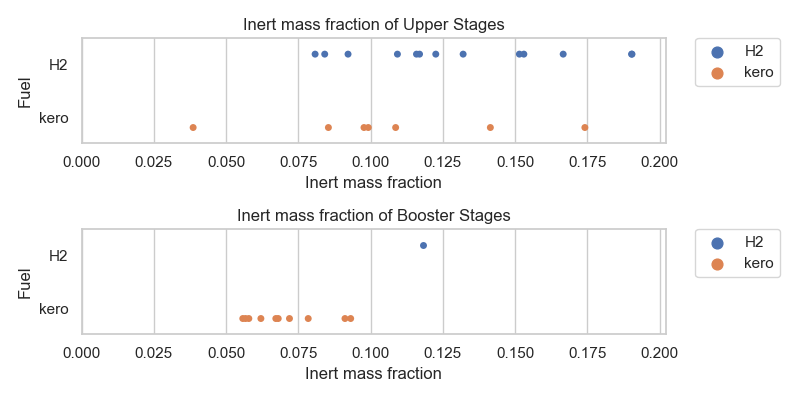
\includegraphics[width=1\textwidth]{stage_trends/stage_inert_mass_fuel}
    \caption{\label{fig:stage_inert_mass_fuel} Stage inert mass fraction by propellant choice.}
\end{figure}

\begin{table}[hbt!]
    \caption{\label{tab:inert_mass_fraction_distributions} Uncertianty distribution parameters on inert mass fraction lower limits.}
    \begin{tabular}{l l c c c}
    \hline
    Stage & Propellant choice & \multicolumn{3}{c}{Triangular dist. params.} \\
    & & Min & Mode & Max \\
    \hline
    \hline
    \multirow{2}{*}{2, Upper} & \ce{H2} / \ce{O2} & 0.080 & 0.085 & 0.090 \\
    & kerosene / \ce{O2} & 0.040 & 0.050 & 0.060 \\
    \multirow{2}{*}{1, Booster} & \ce{H2} / \ce{O2} & 0.110 & 0.120 & 0.130 \\
    & kerosene / \ce{O2} & 0.055 & 0.060 & 0.065 \\
    \hline
    \end{tabular}
\end{table}

\subsection{Recovery Strategy Uncertainties}

\subsubsection{Winged / horizontal landing recovery}
Need to estimate mass of recovery hardware $a$ and recovery propellant $P$.


No winged recovery first stages have actually been operated, so we cannot infer these factors from a sample of historical systems. Instead, we estimate the mass of recovery hardware by three approximate soucres: high-fidelity studies of winged boosters undertaken by major aerospace institutions, a low fidelity study by Barry Hellman of Georgia Tech \cite{Hellman2005}, and analogies to other winged vehicles.

First, we were able to find three high-fidelity winged booster concept designs: Khrunichev's Baikal booster \cite{Isakowitz2004}, NASA/Boeing's Liquid Flyback Booster (dual configuration from \cite{Healy1998}), and DRL's Liquid Flyback Booster \cite{Sippel2003}. These studies list the vehicle inert mass ($m_{inert,1} = m_{s,1} + m_{rh,1}$), the ascent propellant mass ($m_{p,1} - m_{pr,1}$) and the recovery propellant mass ($m_{pr,1}$). We compute $a$ and $P$ as:

\[
a = \frac{m_{inert,1} - m_{p,1} \frac{E_1}{1 - E_1}}{m_{inert,1}}
\]
\[
P = \ln\left( \frac{m_{pr,1}}{m_{inert,1}} + 1 \right)
\]

where $E_1$ is the base expendable inert mass fraction (assumed to be 0.06 for kero/\ce{O2} and 0.12 for \ce{H2}/\ce{O2}), and $m_{p,1} \frac{E_1}{1 - E_1}$ estimates the inert mass of an equivalent expendable stage.

Second, the Hellman study provides estimates of the inert and propellant masses for flyback and glideback boosters. These mass estimates are not based on detailed design considerations, but rather on subsystem mass-estimation relationships developed at Georgia Tech \cite{Rohrschneider2002}.

Our third source is analogy to other winged vehicles. We considered the subsystems which would need to be added to an expendable booster to enable winged recovery (wing, stabiliser, landing gear, surface controls, hydraulics, thermal protection, air breathing propulsion) and computed the fraction of the empty mass is made up by these systems as an estimate of $a$. We considered winged vehicles which cover a variety of missions, sizes and construction technology (STS orbiter, Lockheed C-141, Gulfstream G550, Boeing 787-8).

The resulting estimates of $a$ are shown in Figure \ref{fig:winged_perf_factors}. For powered-flight winged boosters, there is good agreement between the three estimate types. We can have some confidence that $a$ for powered-flight winged boosters is in the range 0.49 to 0.65, i.e. a powered-flight winged booster will have $1/(1-a) =$ 2.0 to 2.8 times the dry mass of an expendable booster with the same propellant load. Glider winged boosters can be expected to be somewhat lighter, with $a$ in the range of 0.38 to 0.54, i.e. having 1.6 to 1.8 times the dry mass of an expendable booster with the same propellant load. We represent the uncertainty on $a$ with a triangular distribution, the parameters of which are given in Table \ref{tab:winged_pref_factor_distributions}.

\begin{figure}[hbt!]
    \centering
    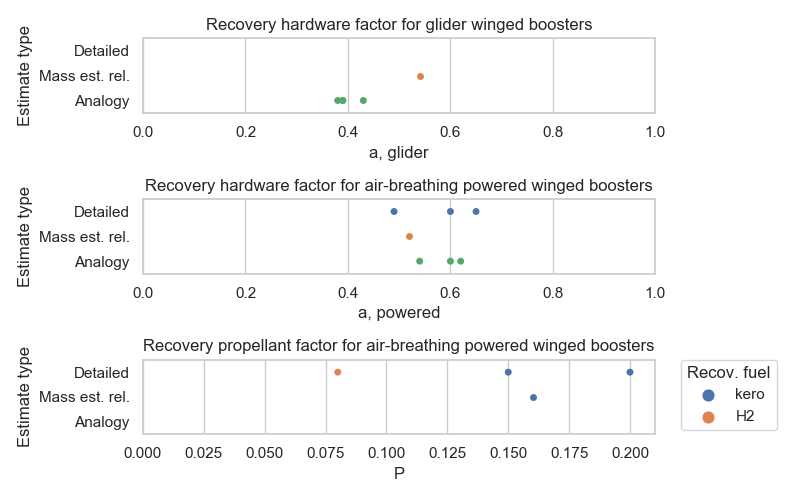
\includegraphics[width=1\textwidth]{recov_strats/winged_perf_factors}
    \caption{\label{fig:winged_perf_factors} Various estimates of the recovery hardware factor $a$ for glider and powered horizontal-landing boosters. Data from \cite{Hellman2005, Isakowitz2004, Healy1998, Sippel2003}}
\end{figure}

\begin{table}[hbt!]
    \centering
    \caption{\label{tab:winged_pref_factor_distributions} Uncertainty distribution parameters of the recovery hardware factor $a$ for glider and powered horizontal-landing boosters.}
    \begin{tabular}{l l c c c}
    \hline
     & \multicolumn{3}{c}{Triangular dist. params.} \\
    & Min & Mode & Max \\
    \hline
    \hline
    Glider  & 0.380 & 0.426 & 0.540 \\
    Powered & 0.490 & 0.574 & 0.650 \\
    \hline
    \end{tabular}
\end{table}

\subsubsection{Propulsive landing}

Need to estimate recovery hardware mass factor $a$.

Propulsive landing boosters require extra hardware not needed on an expendable booster. On most flown or proposed designs, this extra hardware includes aerodynamic control surfaces and actuators, landing gear\footnote{It may be possible to forgo landing gear by high-precision landing on a support structure \cite{Musk2017}, however this difficult technique has yet to be demonstrated.}, and thermal protection \cite{NewGlenn, Falcon9, DCX, Musk2017}.

Although three propulsive landing boosters have been flown, we could not find reliable, publicly available data on the masses of the extra hardware systems. Instead, we will crudely estimate the mass of these systems by analogy to other aerospace vehicles (STS orbiter, Lockheed C-141, Gulfstream G550, Boeing 787-8). On these vehicles, the surface controls and actuators make up 2 to 5\% of the vehicle empty mass, and landing gear 7 to 8\%. Although the design of aircraft landing gear is quite different, this is a decent first guess. We guess that thermal protection adds another 2\% to 4\% (TODO although there is a trade-off against entry burn $\Delta v$). Thus, we expect $a$ to be 0.11 to 0.17, i.e. a propulsive landing booster should have 1.1 to 1.2 times the dry mass of an expendable booster with the same propellant load. Because these estimates are crude, we expand the bounds by 0.02 on either side when choosing the parameters of the triangular distribution (Table \ref{tab:propulsive_pref_factor_distributions}).

\begin{table}[hbt!]
    \centering
    \caption{\label{tab:propulsive_pref_factor_distributions} Uncertainty distribution parameters of the recovery hardware factor $a$ for propulsive-landing boosters.}
    \begin{tabular}{l l c c c}
    \hline
     & \multicolumn{3}{c}{Triangular dist. params.} \\
     & Min & Mode & Max \\
    \hline
    \hline
    Propulsive landing  & 0.09 & 0.14 & 0.19 \\
    \hline
    \end{tabular}
\end{table}


\subsubsection{Parachute recovery}
Need to estimate recovery hardware mass factor $a$.

The Space Shuttle Solid Rocket Boosters (SRBs) and the Ariane 5 EAP boosters are the only operational examples of parachute recovery of full space launch vehicle stages. The mass of the SRB parachutes were 3.5\% of booster dry mass \cite{Wolf1996}, and entry thermal protection added another few percent. Thus, we expect $a$ to be in the range \SIrange{0.05}{0.08}{}.

owever, the SRB example is not indicative of parachute recovery for liquid boosters. Solid rocket boosters must contain a much higher internal pressure than pump-fed liquid stages, and are therefore have a stronger structure which is more robust to entry loads. Attempts to fully recover liquid stages via parachute have failed, with the stages breaking up during reentry \cite{Spencer2011}.

Partial recovery via parachute may be more feasible for liquid boosters, as a compact engine pod could more easily survive entry loads. United Launch Alliance has proposed to recover the engines of Atlas V (or the next-generation Vulcan) via parachutes and mid-air capture \cite{Gravlee2008, Ragab2015}. This proposal also includes an inflatable heat shield (Hypersonic Inflatable Aerodynamic Decelerator, HIAD) which will protect and decelerate the recovery vehicle. The proposed \SI{10}{\meter} HIAD is estimated to have a mass of \SI{1.5}{\mega\gram} \cite{Bose2009}, about 13\% of the recovery vehicle mass. Including parachutes as well, the $a$ value for this strategy should be $\approx 0.17$. Recovery via mid-air capture should reduce recovery operations and refurbishment costs compared to recovery in the ocean.

\begin{table}[hbt!]
    \centering
    \caption{\label{tab:parachute_pref_factor_distributions} Uncertainty distribution parameters of the recovery hardware factor $a$ for parachute recovery boosters.}
    \begin{tabular}{l l c c c}
    \hline
     & \multicolumn{3}{c}{Triangular dist. params.} \\
     & Min & Mode & Max \\
    \hline
    \hline
    Parachutes & 0.050 & 0.065 & 0.080 \\
    Parachutes and inflatable heat shield  & 0.150 & 0.170 & 0.190 \\
    \hline
    \end{tabular}
\end{table}

\section{Cost-Related Uncertainties}



\bibliography{../paper/first_stage_recovery}

\end{document}